\documentclass{standalone}
\usepackage{tikz}
\usetikzlibrary{patterns, positioning}
\usepackage[sfdefault]{ClearSans} %% option 'sfdefault' activates Clear Sans as the default text font
\usepackage[T1]{fontenc}

\begin{document}
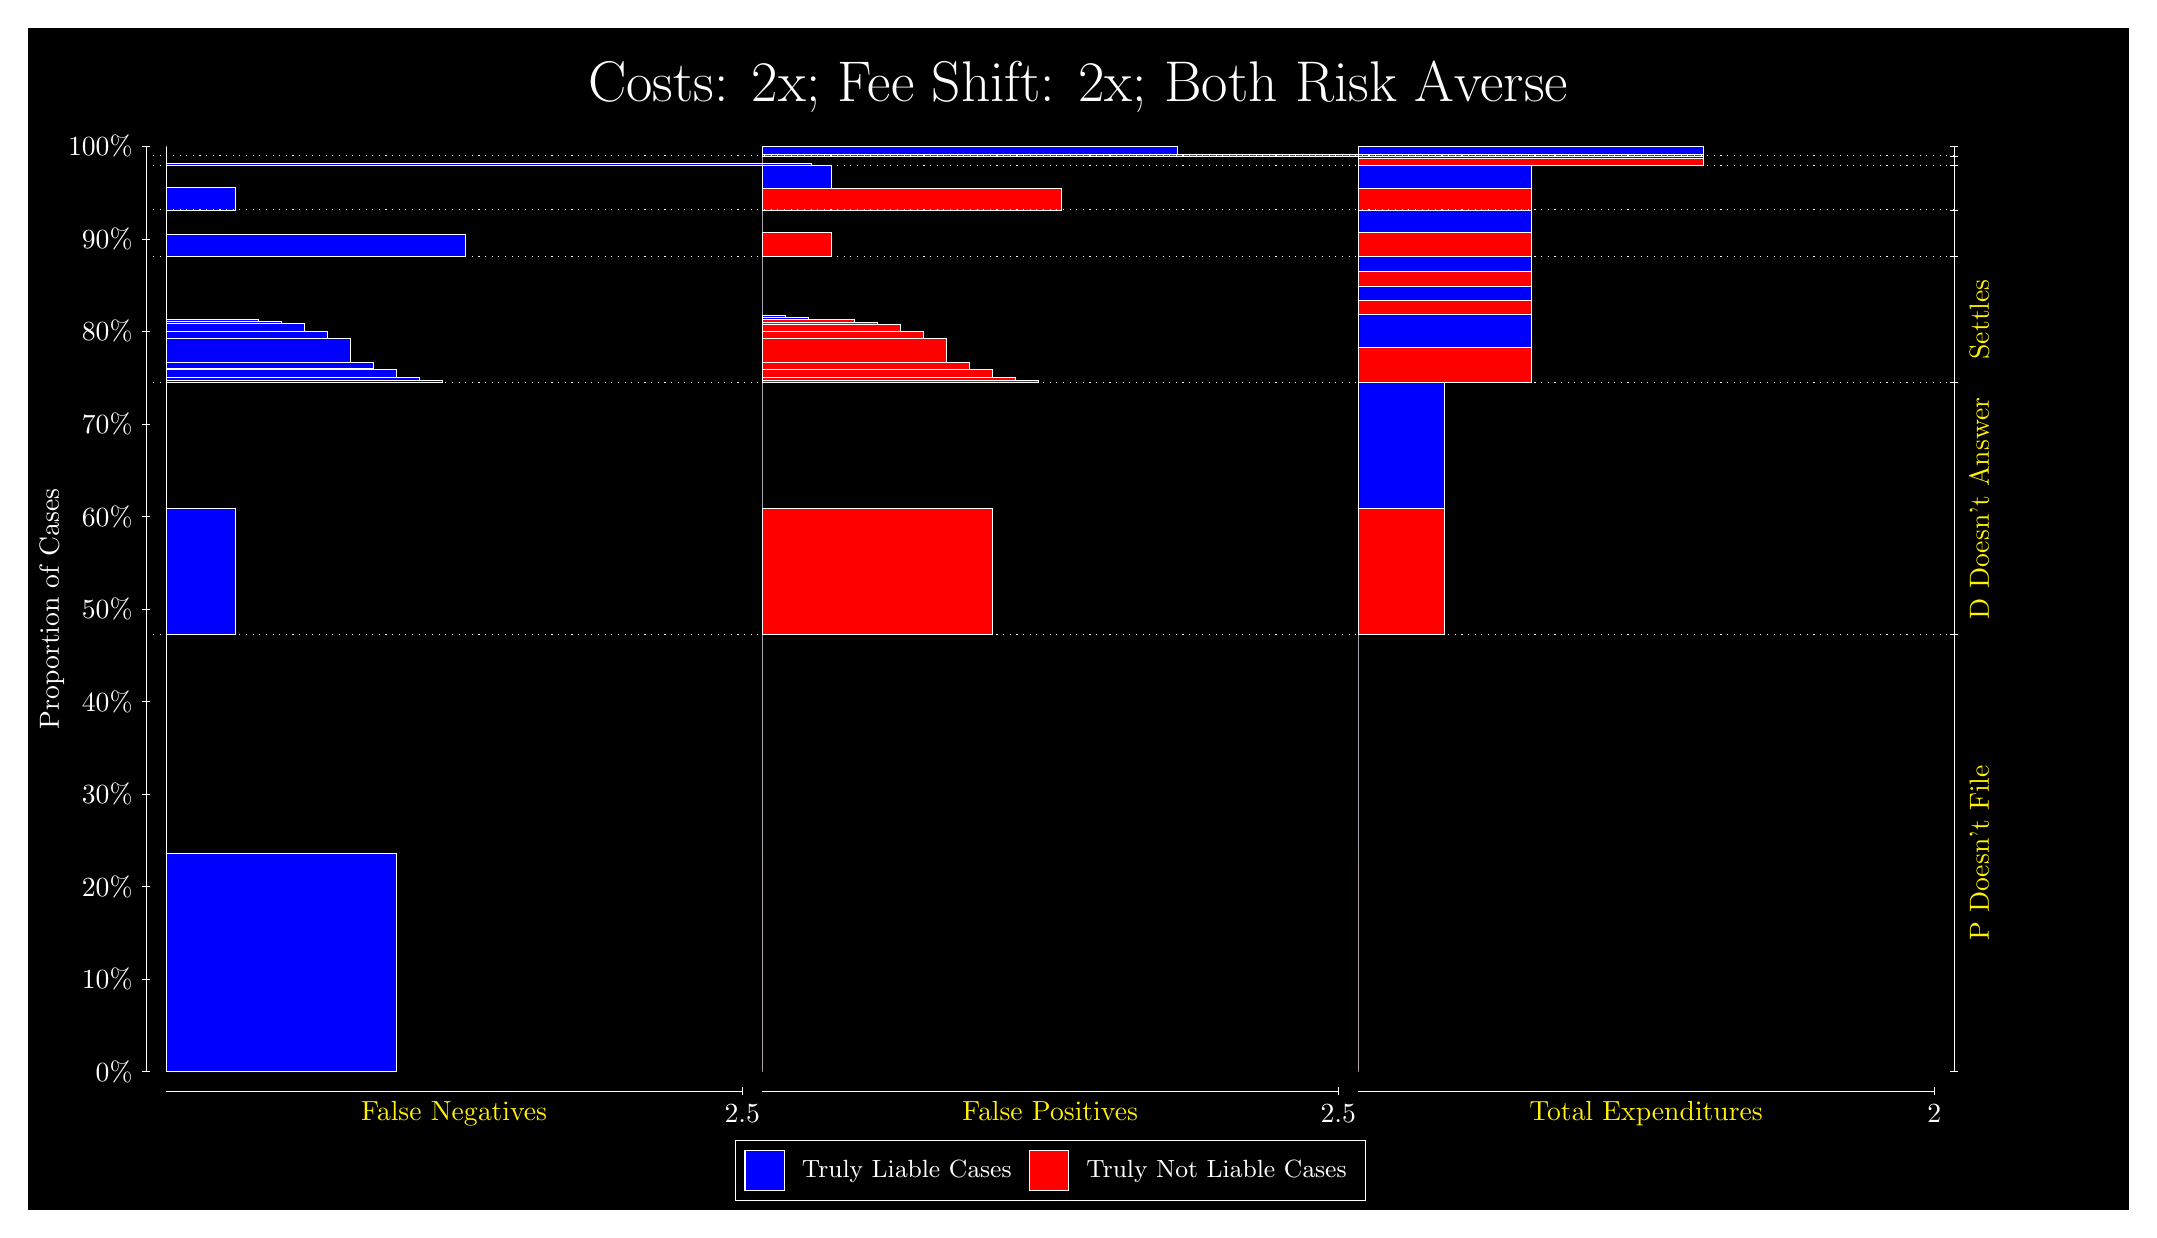
\begin{tikzpicture}
\draw[fill=black] (0,0) rectangle (26.667,15);
\draw[text=white] (0,13.5) rectangle (26.667,15) node[midway] {\huge Costs: 2x; Fee Shift: 2x; Both Risk Averse};
\draw[white, very thin] (1.5,1.75) -- (1.5,13.5);
\node[rotate=90, text=white, anchor=center] at (0.3, 7.625) {Proportion of Cases};
\draw[white, very thin] (1.45,1.75) -- (1.55,1.75);
\node[text=white, anchor=east] at (1.45, 1.75) {0\%};
\draw[white, very thin] (1.45,2.925) -- (1.55,2.925);
\node[text=white, anchor=east] at (1.45, 2.925) {10\%};
\draw[white, very thin] (1.45,4.1) -- (1.55,4.1);
\node[text=white, anchor=east] at (1.45, 4.1) {20\%};
\draw[white, very thin] (1.45,5.275) -- (1.55,5.275);
\node[text=white, anchor=east] at (1.45, 5.275) {30\%};
\draw[white, very thin] (1.45,6.45) -- (1.55,6.45);
\node[text=white, anchor=east] at (1.45, 6.45) {40\%};
\draw[white, very thin] (1.45,7.625) -- (1.55,7.625);
\node[text=white, anchor=east] at (1.45, 7.625) {50\%};
\draw[white, very thin] (1.45,8.8) -- (1.55,8.8);
\node[text=white, anchor=east] at (1.45, 8.8) {60\%};
\draw[white, very thin] (1.45,9.975) -- (1.55,9.975);
\node[text=white, anchor=east] at (1.45, 9.975) {70\%};
\draw[white, very thin] (1.45,11.15) -- (1.55,11.15);
\node[text=white, anchor=east] at (1.45, 11.15) {80\%};
\draw[white, very thin] (1.45,12.325) -- (1.55,12.325);
\node[text=white, anchor=east] at (1.45, 12.325) {90\%};
\draw[white, very thin] (1.45,13.5) -- (1.55,13.5);
\node[text=white, anchor=east] at (1.45, 13.5) {100\%};

\draw[white, very thin] (24.457,1.75) -- (24.457,13.5);
\draw[white, very thin] (24.407,1.75) -- (24.507,1.75);
\node[anchor=west] at (24.407, 1.75) {};
\draw[white, very thin] (24.407,7.3) -- (24.507,7.3);
\node[anchor=west] at (24.407, 7.3) {};
\draw[white, very thin] (24.407,10.503) -- (24.507,10.503);
\node[anchor=west] at (24.407, 10.503) {};
\draw[white, very thin] (24.407,12.104) -- (24.507,12.104);
\node[anchor=west] at (24.407, 12.104) {};
\draw[white, very thin] (24.407,12.692) -- (24.507,12.692);
\node[anchor=west] at (24.407, 12.692) {};
\draw[white, very thin] (24.407,13.255) -- (24.507,13.255);
\node[anchor=west] at (24.407, 13.255) {};
\draw[white, very thin] (24.407,13.379) -- (24.507,13.379);
\node[anchor=west] at (24.407, 13.379) {};
\draw[white, very thin] (24.407,13.5) -- (24.507,13.5);
\node[anchor=west] at (24.407, 13.5) {};

\draw[white, very thin, fill=blue] (1.75,1.75) rectangle (4.6775,4.525);
\draw[white, very thin, fill=red] (1.75,4.525) rectangle (1.75,7.3);
\draw[white, very thin, fill=blue] (1.75,7.3) rectangle (2.6283,8.9013);
\draw[white, very thin, fill=red] (1.75,8.9013) rectangle (1.75,10.503);
\draw[white, very thin, fill=blue] (1.75,10.503) rectangle (5.2631,10.535);
\draw[white, very thin, fill=blue] (1.75,10.535) rectangle (4.9703,10.563);
\draw[white, very thin, fill=blue] (1.75,10.563) rectangle (4.6775,10.663);
\draw[white, very thin, fill=blue] (1.75,10.663) rectangle (4.3848,10.682);
\draw[white, very thin, fill=blue] (1.75,10.682) rectangle (4.3848,10.755);
\draw[white, very thin, fill=blue] (1.75,10.755) rectangle (4.092,11.065);
\draw[white, very thin, fill=blue] (1.75,11.065) rectangle (3.7993,11.154);
\draw[white, very thin, fill=blue] (1.75,11.154) rectangle (3.5065,11.25);
\draw[white, very thin, fill=blue] (1.75,11.25) rectangle (3.2138,11.276);
\draw[white, very thin, fill=blue] (1.75,11.276) rectangle (2.921,11.306);
\draw[white, very thin, fill=red] (1.75,11.306) rectangle (1.75,12.104);
\draw[white, very thin, fill=blue] (1.75,12.104) rectangle (5.5558,12.389);
\draw[white, very thin, fill=red] (1.75,12.389) rectangle (1.75,12.692);
\draw[white, very thin, fill=blue] (1.75,12.692) rectangle (2.6283,12.981);
\draw[white, very thin, fill=red] (1.75,12.981) rectangle (1.75,13.255);
\draw[white, very thin, fill=blue] (1.75,13.255) rectangle (9.9471,13.28);
\draw[white, very thin, fill=red] (1.75,13.28) rectangle (1.75,13.379);
\draw[white, very thin, fill=red] (1.75,13.379) rectangle (1.75,13.404);
\draw[white, very thin, fill=blue] (1.75,13.404) rectangle (1.75,13.5);
\draw[white, very thin, fill=red] (9.3189,1.75) rectangle (9.3189,4.5251);
\draw[white, very thin, fill=blue] (9.3189,4.5251) rectangle (9.3189,7.3);
\draw[white, very thin, fill=red] (9.3189,7.3) rectangle (12.246,8.9014);
\draw[white, very thin, fill=blue] (9.3189,8.9014) rectangle (9.3189,10.503);
\draw[white, very thin, fill=red] (9.3189,10.503) rectangle (12.832,10.533);
\draw[white, very thin, fill=red] (9.3189,10.533) rectangle (12.539,10.561);
\draw[white, very thin, fill=red] (9.3189,10.561) rectangle (12.246,10.664);
\draw[white, very thin, fill=red] (9.3189,10.664) rectangle (11.954,10.759);
\draw[white, very thin, fill=red] (9.3189,10.759) rectangle (11.661,11.067);
\draw[white, very thin, fill=red] (9.3189,11.067) rectangle (11.368,11.151);
\draw[white, very thin, fill=red] (9.3189,11.151) rectangle (11.075,11.243);
\draw[white, very thin, fill=red] (9.3189,11.243) rectangle (10.783,11.269);
\draw[white, very thin, fill=red] (9.3189,11.269) rectangle (10.49,11.3);
\draw[white, very thin, fill=blue] (9.3189,11.3) rectangle (9.9044,11.331);
\draw[white, very thin, fill=blue] (9.3189,11.331) rectangle (9.6116,11.357);
\draw[white, very thin, fill=blue] (9.3189,11.357) rectangle (9.3189,12.104);
\draw[white, very thin, fill=red] (9.3189,12.104) rectangle (10.197,12.407);
\draw[white, very thin, fill=blue] (9.3189,12.407) rectangle (9.3189,12.692);
\draw[white, very thin, fill=red] (9.3189,12.692) rectangle (13.125,12.967);
\draw[white, very thin, fill=blue] (9.3189,12.967) rectangle (10.197,13.255);
\draw[white, very thin, fill=red] (9.3189,13.255) rectangle (9.3189,13.354);
\draw[white, very thin, fill=blue] (9.3189,13.354) rectangle (9.3189,13.379);
\draw[white, very thin, fill=red] (9.3189,13.379) rectangle (17.516,13.404);
\draw[white, very thin, fill=blue] (9.3189,13.404) rectangle (14.588,13.5);
\draw[white, very thin, fill=red] (16.888,1.75) rectangle (16.888,4.5251);
\draw[white, very thin, fill=blue] (16.888,4.5251) rectangle (16.888,7.3);
\draw[white, very thin, fill=red] (16.888,7.3) rectangle (17.986,8.9014);
\draw[white, very thin, fill=blue] (16.888,8.9014) rectangle (17.986,10.503);
\draw[white, very thin, fill=red] (16.888,10.503) rectangle (19.083,10.942);
\draw[white, very thin, fill=blue] (16.888,10.942) rectangle (19.083,11.373);
\draw[white, very thin, fill=red] (16.888,11.373) rectangle (19.083,11.541);
\draw[white, very thin, fill=blue] (16.888,11.541) rectangle (19.083,11.72);
\draw[white, very thin, fill=red] (16.888,11.72) rectangle (19.083,11.911);
\draw[white, very thin, fill=blue] (16.888,11.911) rectangle (19.083,12.104);
\draw[white, very thin, fill=red] (16.888,12.104) rectangle (19.083,12.407);
\draw[white, very thin, fill=blue] (16.888,12.407) rectangle (19.083,12.692);
\draw[white, very thin, fill=red] (16.888,12.692) rectangle (19.083,12.967);
\draw[white, very thin, fill=blue] (16.888,12.967) rectangle (19.083,13.255);
\draw[white, very thin, fill=red] (16.888,13.255) rectangle (21.279,13.354);
\draw[white, very thin, fill=blue] (16.888,13.354) rectangle (21.279,13.379);
\draw[white, very thin, fill=red] (16.888,13.379) rectangle (21.279,13.404);
\draw[white, very thin, fill=blue] (16.888,13.404) rectangle (21.279,13.5);
\draw[white, dotted] (1.5,7.3) -- (24.457,7.3);
\draw[white, dotted] (1.5,10.503) -- (24.457,10.503);
\draw[white, dotted] (1.5,12.104) -- (24.457,12.104);
\draw[white, dotted] (1.5,12.692) -- (24.457,12.692);
\draw[white, dotted] (1.5,13.255) -- (24.457,13.255);
\draw[white, dotted] (1.5,13.379) -- (24.457,13.379);
\draw[white, very thin] (1.75,1.5) -- (9.0689,1.5);
\node[text=yellow, anchor=north] at (5.4094, 1.5) {False Negatives};
\draw[white, very thin] (9.0689,1.45) -- (9.0689,1.55);
\node[text=white, anchor=north] at (9.0689, 1.45) {2.5};

\draw[white, very thin] (9.3189,1.5) -- (16.638,1.5);
\node[text=yellow, anchor=north] at (12.978, 1.5) {False Positives};
\draw[white, very thin] (16.638,1.45) -- (16.638,1.55);
\node[text=white, anchor=north] at (16.638, 1.45) {2.5};

\draw[white, very thin] (16.888,1.5) -- (24.207,1.5);
\node[text=yellow, anchor=north] at (20.547, 1.5) {Total Expenditures};
\draw[white, very thin] (24.207,1.45) -- (24.207,1.55);
\node[text=white, anchor=north] at (24.207, 1.45) {2};

\node[text=yellow, centered, rotate=90] at (24.777, 4.525) {P Doesn't File};
\node[text=yellow, centered, rotate=90] at (24.777, 8.9014) {D Doesn't Answer};
\node[text=yellow, centered, rotate=90] at (24.777, 11.303) {Settles};





\draw (12.978300999999998,1.5) node[draw=none] (baseCoordinate) {};
\begin{scope}[align=center]
        \matrix[scale=0.5, draw=white, below=0.5cm of baseCoordinate, nodes={draw}, column sep=0.1cm]{
            \node[rectangle, draw, minimum width=0.5cm, minimum height=0.5cm, fill=blue] {}; &
            \node[draw=none, font=\small, text=white] (B) {Truly Liable Cases}; &
            \node[rectangle, draw, minimum width=0.5cm, minimum height=0.5cm, fill=red] {}; &
            \node[draw=none, font=\small, text=white] (B) {Truly Not Liable Cases}; \\
            };
\end{scope}

\end{tikzpicture}
\end{document}